\documentclass[letterpaper,11pt]{article}
\usepackage{amsmath, amsthm, amssymb}
\usepackage{bridges}
\usepackage{graphicx}

\usepackage[colorlinks=true, urlcolor=blue, citecolor=black, linkcolor=black]{hyperref}
%\usepackage{subcaption}

\usepackage{algorithm}
\usepackage{algpseudocode}
%\usepackage{hyperref} % already loaded above

%\usepackage{svg}
%\usepackage{multirow}
%\usepackage{caption}
%\usepackage{tikz}
%\usepackage{transparent}

%\usepackage[bottom]{footmisc}

\urlstyle{rm}

\newtheorem{lemma}{Lemma}

%\sloppy
\usepackage{listings}
%\lstset{breaklines=true}

\title{ A Generalized 2D and 3D Hilbert Curve }
\author{ Jakub \v{C}erven\'{y} and Zzyv Zzyzek }

\date{}

\begin{document}

\maketitle

\thispagestyle{empty}

\begin{abstract}
  Hilbert curves are classic space-filling curves with strong locality properties, widely
  used for linearizing 2D and 3D data. In their discrete form, however, the standard
  Hilbert construction applies most naturally to square or cubic grids with side lengths
  that are exact powers of two.
  We present the \emph{Gilbert curve}, a simple recursive, Hilbert-like construction that
  produces Hamiltonian paths on \emph{arbitrary} 2D and \emph{even-sized} 3D axis-aligned rectangular grids.
  Our construction explicitly manages endpoint parity constraints, and extends naturally
  to 3D.
\end{abstract}


\section*{Introduction}

%\paragraph{Contributions}

Space-filling curves map a one-dimensional ordering to a multi-dimensional grid while
preserving locality.
%as much as possible.
Discrete Hilbert curves, in particular,
%are commonly
can be
used to linearize images or volumes for cache-coherent traversal,
construct spatial indexes, visualize data layout, and more \cite{anders2009, bohm2021, cortesi2011, moon2001, munroe2006}.
In practical settings, however, underlying grids might not be square or cubic with
power-of-two side lengths. Images and volumes can come in arbitrary dimensions;
tiling, padding, or resampling to fit a power-of-two Hilbert curve introduces overhead
and can harm locality near boundaries.


\begin{figure}[!htb]
  \begin{minipage}{0.48\textwidth}
    \centering
    \includegraphics[width=\linewidth]{gilbert2d_examples.pdf}
    \caption{2D Gilbert curves for i) $8\times 8$, ii) $18\times 6$, iii) $13\times 8$ (with notch), iv) $14\times 14$.}
    \label{fig:gilbert2d_examples}
  \end{minipage}\hfill
  \begin{minipage}{0.46\textwidth}
    \centering
    \includegraphics[width=\linewidth]{gilbert3d_orig_examples.pdf}
    \caption{3D Gilbert curves for i) $4 \times 4 \times 4$, ii) $6 \times 6 \times 6$, iii) $8 \times 4 \times 4$, iv) $5  \times 4 \times 4$ (with notch).}
    \label{fig:examples3d}
  \end{minipage}
\end{figure}


This paper presents the \emph{Gilbert curve}, a recursive construction that produces a
Hamiltonian path (a non-self-intersecting path visiting every grid vertex exactly once)
on arbitrary 2D rectangles and 3D cuboids.
Our goal is a construction that is easy to implement, has a uniform recursive structure,
and reduces to the standard Hilbert curve in the power-of-two square/cube cases.
In this paper, we:

\begin{itemize}
  \item We describe a simple recursive construction of Hilbert-like
        %Hamiltonian
        paths on
        arbitrary 2D rectangular grids
  \item We formalize a parity
        %(``color compatibility'')
        condition on corner endpoints and
        use it to guide valid recursive subdivisions
  \item We extend the same construction principles naturally to arbitrary 3D cuboid grids
        %, reusing the 2D routine for planar subproblems.
\end{itemize}

%\begin{figure}[!htb]
%  \centering
%  \includegraphics[width=\linewidth]{simple_hampath_flat.pdf}
%  \caption{Hamiltonian path feasibility for small grids. A red `x' marks a corner endpoint that is impossible given the chosen start.}
%  \label{fig:exampleHampath}
%\end{figure}



\section*{Related Work}

Hilbert introduced his eponymous curve as a continuous mapping from the unit interval to the unit square \cite{hilbert1891}.
Many discrete variants exist; the most common recursive discretization applies most directly to
power-of-two square (2D) and cubic (3D) grids.

Tautenhahn \cite{lutanho2003} presents an unpublished 2D construction for arbitrary sizes based on combining
$3\times3$ Peano and $2\times2$ Hilbert block types. While that approach is 2D-only and not purely uniform across scales,
it motivates an important endpoint-parity constraint that we make explicit. % in Section~\ref{sec:parity}.

Zhang, Kamata, and Ueshige \cite{zhang2006} propose a pseudo-Hilbert scan for arbitrary rectangles.
Compared to our construction, their method follows a more intricate case structure and does not
suggest a direct extension to 3D.

%\section{Examples}
%
%Figure~\ref{fig:gilbert2d_examples} shows 2D Gilbert curves on a square grid, an eccentric rectangle,
%and a rectangle with a small notch. Figure~\ref{fig:examples3d} shows analogous 3D examples.

\section*{Parity Constraints on Corner Endpoints}
\label{sec:parity}

%\begin{figure}[!htb]
%
%  \begin{minipage}{0.48\textwidth}
%
%    \centering
%    %\begin{table}[h]
%    %  \centering
%      \begin{tabular}[t]{cr|cc}
%        \multicolumn{2}{c}{ \multirow{2}{*}{Path Possible} } & \multicolumn{2}{c}{Volume} \\
%        & & \textit{even} & \textit{odd} \\
%        \hline
%          %\multirow{2}{*}{$|\alpha| \bmod 2$} & \textit{even} & Yes & Yes \\
%          \multirow{2}{*}{ $|\alpha|$ } & \textit{even} & Yes & Yes \\
%           & \textit{odd} & \textbf{No} & Yes \\
%         \hline
%      \end{tabular}
%      \caption{ $|\alpha|$ is the distance of endpoints.
%                A Hamiltonian path is possible only when $|\alpha|$ is even or both
%                $|\alpha|$ and the volume are odd. }
%      \label{table:pathTable}
%    %\end{table}
%
%  \end{minipage}\hfill
%  \begin{minipage}{0.48\textwidth}
%
%    \centering
%    \includegraphics[width=\linewidth]{simple_hampath.pdf}
%    \caption{ Examples of Hamiltonian paths for small grid sizes. A red `x' corresponds to no possible path for the chosen endpoints. }
%    \label{fig:exampleHampath}
%
%  \end{minipage}
%
%\end{figure}

We will repeatedly need to know when a Hamiltonian path is possible between two corners of a grid.
The key constraint is parity. Consider the standard checkerboard coloring of an $m\times n$ grid graph (or an $m\times n\times p$ grid graph in 3D):
adjacent vertices always have opposite color.
Any path alternates colors at every step, so the parity of the endpoints is constrained by the total number of visited vertices.

\begin{lemma}[Color compatibility]
  \label{lemma:colorCompatibility}
Let $G$ be a rectangular 2D grid graph with $mn$ vertices, or a rectangular 3D grid graph with $mnp$ vertices.
Fix a start corner $s$ and an end corner $t$.
If there exists a Hamiltonian path from $s$ to $t$, then $s$ and $t$ have the \emph{same} color when the number of vertices is odd,
and \emph{opposite} colors when the number of vertices is even.
\end{lemma}

\begin{proof}
Along any path, vertex colors alternate. A Hamiltonian path visits all $N$ vertices exactly once and therefore has $N-1$ steps.
If $N$ is odd, then $N-1$ is even and the endpoints must have the same color; if $N$ is even, then $N-1$ is odd and the endpoints must have opposite colors.
\end{proof}

We call a pair of endpoints \emph{color compatible} if they satisfy the lemma.
%Figure~\ref{fig:exampleHampath} illustrates the constraint for small 2D grids.
Color compatibility is necessary in general; for the specific family of corner-to-corner subproblems produced by our construction,
it is also sufficient, and we use it as a lightweight validity check when selecting subdivisions.

%For a path starting at $(0,0,0)$ and ending $|\alpha|$ steps in one of the axis-aligned dimensions,
%then Table \ref{table:pathTable} enumerates this condition under which a valid path is possible.

%Assuming a curve starts from position $p_s=(0,0,0)$ and has proposed
%endpoint at $p_e=((w-1),0,0)$, with a cuboid region as $\alpha = (w,0,0), \beta = (0,h,0), \gamma = (0,0,d)$.

%We focus on optimizing for providing a notch-free path when all side lengths are even and allow notches when $|\alpha|$ is odd in 2D
%or when one of the side lengths is odd in 3D.

%The 2D Gilbert curve limits the number of notches to one.
%The 3D Gilbert curve's subdivision strategy creates a notch when the distance between endpoints is odd,
%potentially creating more than one notch.
%
%In both the 2D and 3D case, when the original side lengths are all even, no notches will be present.
%



\begin{figure}[!htb]

  \begin{minipage}{0.55\textwidth}

    \begin{minipage}{1.0\textwidth}
      \centering
      \includegraphics[width=\linewidth]{gilbert2d_mainsubdiv.pdf}
      \caption{ Subdivision template for the 2D Gilbert curve. }
      \label{fig:main2dsubdiv}
    \end{minipage}

    \begin{minipage}{1.0\textwidth}
      \centering
      \includegraphics[width=0.65\linewidth]{gilbert2d_example_mainsubdiv.pdf}
      \caption{ Example curve with subdivision regions highlighted. }
      \label{fig:main2dsubdivExample}
    \end{minipage}

  \end{minipage}\hfill
  \begin{minipage}{0.45\textwidth}
    \centering
    \includegraphics[width=\linewidth]{gilbert3d_explode.pdf}
    \caption{ The main subdivision template for the 3D Gilbert curve. }
    \label{fig:gilbert3DJSplit}
  \end{minipage}

\end{figure}

\section*{The 2D Gilbert Curve}
\label{sec:2d}

Our 2D construction recursively partitions an $m\times n$ rectangle into a small number of axis-aligned sub-rectangles
and concatenates the subpaths into a single Hamiltonian path.
Figure~\ref{fig:main2dsubdiv} shows the main 2D subdivision template and
Figure~\ref{fig:main2dsubdivExample} illustrates one recursion with subregions highlighted.

The vectors $\alpha, \beta, \gamma \in \mathbb{Z}^3$ provide generalized notions of width ($\alpha$), height ($\beta$),
and depth ($\gamma$), so that we can transform rectangular or cuboid regions as necessary for the recursion.
Each of $\alpha, \beta, \gamma$ will only have one non-zero component and will be orthogonal to each other,
representing a snapshot of the current frame of reference.

When dividing into subregions, we choose integral side lengths and prefer even lengths, where possible, to satisfy the
parity constraints of lemma \ref{lemma:colorCompatibility}. %Section~\ref{sec:parity}.
Each subregion is solved recursively and then stitched to its neighbors.
%Figure~\ref{fig:production2d} summarizes the main parity-driven cases.

When one side length is much larger than the other, we optionally apply an \emph{eccentric split} that first bisects the long side.
This improves robustness on highly elongated rectangles and keeps the recursion structure simple.


%\subsection*{2D Gilbert Curve}
%
%For the 2D Gilbert curve,
%the region is subdivided into two squares at the bottom and a rectangle on top, with endpoints
%joined on the outer perimeter.
%This process is recursively applied until a trivial path can be produced.
%Figures \ref{fig:main2dsubdiv} and \ref{fig:gilbert2d_bulk} show two different representations of the template used for the
%subdivision.
%Figures \ref{fig:main2dsubdivExample} and \ref{fig:gilbert2d_bulk_example} show color coded examples for dimensions $26 \times 18$ and
%$42 \times 30$ respectively.
%
%If the width like dimension ($\alpha$) is much larger than the height like dimension ($\beta$),
%an alternate eccentric subdivision template is used to split the region in half along
%the $\alpha$ length (figure \ref{fig:eccentric_2d_alg}, \ref{fig:eccentric_2d_example_alg}).
%
%Each regions parity is chosen so as to try and keep color compatibility, ensuring a valid path if possible.
%If the $\alpha$ axis line that the endpoints fall on is odd, with the orthogonal $\beta$ direction even, a notch is forced and is directed to the upper right region,
%as illustrated by the ``even/odd'' case in figure \ref{fig:production2d}.

When the side lengths are exact powers of two, the resulting curve is identical to the 2D Hilbert curve.

%\begin{figure}[!htb]
%  \centering
%  \includegraphics[width=\linewidth]{config_production.pdf}
%  \caption{ Enumeration of the subdivision template depending on different parities of $\alpha$ and $\beta$ dimensions. }
%  \label{fig:production2d}
%\end{figure}


\section*{Extension to 3D}
\label{sec:3d}

In the normal case, a subdivision scheme is used to split the cuboid into five regions.
Two cube like regions are partitioned where the path starts and stops, and three oblong cuboid regions are partitioned
for the middle portion of the path.
Figure \ref{fig:gilbert3DJSplit} provides an exploded view of the main subdivision and where the endpoints line up.
See also figure \ref{fig:gilbert3d_bulk_template} for the template and Figure \ref{fig:gilbert3d_bulk_example}
for a $10 \times 10 \times 10$ example, with each region color coded.

Endpoints within a sub-divided region are kept on the exterior of the parent cuboid and joined after the resulting recursion
has completed.
As with the 2D Gilbert curve, when side dimensions are equal and exact powers of two, the resulting curve is identical to the
corresponding 3D Hilbert curve.

During the course of sub-division, if the width like dimension ($\alpha$) is much larger, the curve is split in half along
the $\alpha$ length (Figure \ref{fig:gilbert3d_eccentric_alpha}, \ref{fig:gilbert3d_eccentric_alpha_example}).
If the $\alpha$ eccentric split is not triggered, the height-like dimension, $\beta$, is then compared to the depth-like dimension, $\gamma$
and, if very much larger, an eccentric subdivision scheme is used that splits in the $\alpha$ and $\beta$ direction
(Figure \ref{fig:gilbert3d_eccentric_beta}, \ref{fig:gilbert3d_eccentric_beta_example}).
If both $\alpha$ and $\beta$ are not much larger, a check is done to see if the depth-like dimension, $\gamma$, is much larger than
than the height-like dimension, $\beta$, splitting in the $\alpha$ and $\gamma$ direction if so
(Figure \ref{fig:gilbert3d_eccentric_gamma}, \ref{fig:gilbert3d_eccentric_gamma_example}).

If any of the subdivided regions has endpoints that lay in a direction with
odd length, a notch will appear.
This means the number of notches for the 3D Gilbert curve isn't limited to one in the case a side length is odd.

In the case all side lengths are even, the subdivision will always choose an even length until the base case is
encountered, ensuring a notch-free realization.

\section*{Algorithms}
\label{sec:algorithms}

Algorithms~\ref{alg:gilbert2d} and~\ref{alg:gilbert3d} give pseudocode for the 2D and 3D constructions.
We represent an oriented grid-aligned rectangle or cuboid by an origin $p\in\mathbb{Z}^3$ and axis vectors
$\alpha,\beta,\gamma\in\mathbb{Z}^3$ whose nonzero components encode the side lengths and directions.
The function $\delta(\cdot)$ returns the unit axis direction of its argument, and $\text{div}(\cdot,\cdot)$ denotes
integer division (rounding toward zero).
Eccentric splits are triggered by simple aspect-ratio thresholds in the pseudocode.

\begin{minipage}[!htb]{0.43\linewidth}
\begin{algorithm}[H]
  \caption{Gilbert 2D}
  \label{alg:gilbert2d}
  \begin{algorithmic}

    \State \textit{\# $p, \alpha, \beta \in \mathbb{Z}^3$}
    \Function{Gilbert2D}{$p$, $\alpha$, $\beta$}
      \State $\alpha_2, \beta_2  = \text{div}(\alpha, 2), \text{div}(\beta, 2)$
      \If{ $(|\beta| \equiv 1)$ }
        \State \textbf{yield} $p + i \cdot \delta(\alpha)$ \textbf{forall} $i \in |\alpha|$
      \ElsIf{ $(|\alpha| \equiv 1)$ }
        \State \textbf{yield} $p + i \cdot \delta(\beta)$ \textbf{forall} $i \in |\beta|$
      \ElsIf{ $(2 |\alpha| > 3 |\beta|)$ }
        \If{ $(|\alpha_2| > 2)$ and \\ \hskip4.12em $(|\alpha_2| \bmod{2} \equiv 1)$ }
          \State $\alpha_2 \leftarrow \alpha_2 + \delta(\alpha)$
        \EndIf
        \State \textbf{yield} Gilbert2D($p$, $\alpha_2$, $\beta$)
        \State \textbf{yield} Gilbert2D($p + \alpha_2$, $\alpha - \alpha_2$, $\beta$)
      \Else
        \If{ $(|\beta_2| > 2)$ and \\ \hskip4.12em $(|\beta_2| \bmod{2} \equiv 1)$ }
          \State $\beta_2 \leftarrow \beta_2 + \delta(\beta)$
        \EndIf
        \State \textbf{yield} Gilbert2D($p$, \\ \hskip9.75em $\beta_2$, $\alpha_2$)
        \State \textbf{yield} Gilbert2D($p + \beta_2$, \\ \hskip9.75em $\alpha$, $(\beta - \beta_2)$)
        \State \textbf{yield} Gilbert2D($p + (\alpha - \delta(\alpha)) +$ \\ \hskip9.75em $(\beta_2 - \delta(\beta))$, \\ \hskip9.75em $-\beta_2$, $-(\alpha - \alpha_2)$)
      \EndIf
    \EndFunction

  \end{algorithmic}
\end{algorithm}
\end{minipage}\hfill
\begin{minipage}[!htb]{0.43\linewidth}

  \begin{minipage}[ht]{0.49\linewidth}

    \centering
    \includegraphics[width=0.925\linewidth]{gilbert2d_eccentric_alpha1.pdf}
    \captionof{figure}{ }
    \label{fig:eccentric_2d_alg}

  \end{minipage}\hfill
  \begin{minipage}[ht]{0.47\linewidth}

    \centering
    \includegraphics[width=1.0\linewidth]{gilbert2d_example_eccentric.pdf}
    \captionof{figure}{ }
    \label{fig:eccentric_2d_example_alg}

  \end{minipage}

  \begin{minipage}[ht]{0.95\linewidth}

    \centering
    \includegraphics[width=0.925\linewidth]{gilbert2d_bulk.pdf}
    \captionof{figure}{ }
    \label{fig:gilbert2d_bulk}

  \end{minipage}

  \begin{minipage}[ht]{0.95\linewidth}

    \centering
    \includegraphics[width=1.0\linewidth]{gilbert2d_bulk_example.pdf}
    \captionof{figure}{ }
    \label{fig:gilbert2d_bulk_example}

  \end{minipage}

\end{minipage}






% (Discussion of ``harmony'' and defect-based eccentric-split tuning omitted from the main paper;
% see Section~\ref{sec:outlook} for a brief outlook.)



\begin{minipage}[ht]{0.5\linewidth}
\begin{algorithm}[H]
  \caption{Gilbert 3D}
  \label{alg:gilbert3d}
  \begin{algorithmic}

    \State \textit{\# $p, \alpha, \beta, \gamma \in \mathbb{Z}^3$}
    \Function{Gilbert3D}{$p$, $\alpha$, $\beta$, $\gamma$}

    \State \Return Gilbert2D($p$,$\beta$,$\gamma$) \textbf{if} $(|\alpha| \equiv 1)$
    \State \Return Gilbert2D($p$,$\alpha$,$\gamma$) \textbf{if} $(|\beta| \equiv 1)$
    \State \Return Gilbert2D($p$,$\alpha$,$\beta$) \textbf{if} $(|\gamma| \equiv 1)$

    \State $\alpha_2 \leftarrow \text{div}(\alpha,2) + \Delta(\alpha _ 2, \alpha)$
    \State $\beta_2 \leftarrow \text{div}(\beta,2) + \Delta(\beta _ 2, \beta)$
    \State $\gamma_2 \leftarrow \text{div}(\gamma,2) + \Delta(\gamma _ 2, \gamma)$

    \State \textbf{if }$(2 |\alpha|>3|\beta|) \text{ and } (2|\alpha|>3|\gamma|))$
    \State \hskip1.0em \textbf{yield} Gilbert3D($p$,$\alpha _ 2$,$\beta$,$\gamma$)
    \State \hskip1.0em \textbf{yield} Gilbert3D($p + \alpha _ 2$,$\alpha - \alpha _ 2$,$\beta$,$\gamma$)
    \State \textbf{else if }$(3 |\beta| > 4 |\gamma|)$
    \State \hskip1.0em \textbf{yield} Gilbert3D($p$,$\beta _ 2$,$\gamma$,$\alpha _ 2$)
    \State \hskip1.0em \textbf{yield} Gilbert3D($p + \beta _ 2$,$\alpha$,$\beta - \beta _ 2$,$\gamma$)
    \State \hskip1.0em \textbf{yield} Gilbert3D($p + $ \\ \hskip9.125em $(\alpha - \delta(\alpha)) +$ \\ \hskip9.125em $(\beta _ 2 - \delta(\beta))$, \\ \hskip9.125em $-\beta _ 2$,$\gamma$,$-(\alpha - \alpha _ 2)$)
    \State \textbf{else if }$(3 |\gamma| > 4 |\beta|)$
    \State \hskip1.0em \textbf{yield} Gilbert3D($p$,$\gamma _ 2$,$\alpha _ 2$,$\beta$)
    \State \hskip1.0em \textbf{yield} Gilbert3D($p + \gamma _ 2$,$\alpha$, $\beta$, $\gamma - \gamma _ 2$)
    \State \hskip1.0em \textbf{yield} Gilbert3D($p +$ \\ \hskip9.125em $(\alpha - \delta(\alpha))$ \\ \hskip9.125em $(\gamma2 - \delta(\gamma))$, \\ \hskip9.5em $-\gamma _ 2$,$-(\alpha-\alpha _ 2)$, $\beta$)

    \State
    \State \textbf{else }
    \State \hskip1.0em \textbf{yield} Gilbert3D($p$,$\beta _ 2$,$\gamma _ 2$,$\alpha _ 2$)
    \State \hskip1.0em \textbf{yield} Gilbert3D($p + \beta _ 2$,$\gamma$,$\alpha _ 2$,$(\beta - \beta _ 2)$)
    \State \hskip1.0em \textbf{yield} Gilbert3D($p +$ \\ \hskip9.125em $(\beta _ 2 - \delta(\beta)) +$ \\ \hskip9.125em $(\gamma - \delta(\gamma))$, \\ \hskip9.5em $\alpha$,$-\beta_2$,$-(\gamma-\gamma_2)$)
    \State \hskip1.0em \textbf{yield} Gilbert3D($p +$ \\ \hskip9.125em $(\alpha _ 2 - \delta(\alpha)) +$ \\ \hskip9.125em $\beta _ 2 + (\gamma - \delta(\gamma))$, \\ \hskip9.5em $-\gamma$,$-(\alpha - \alpha_2)$,$(\beta-\beta_2)$)
    \State \hskip1.0em \textbf{yield} Gilbert3D($p +$ \\ \hskip9.125em $(\alpha - \delta(\alpha)) +$ \\ \hskip9.125em $(\beta _ 2 - \delta(\beta))$, \\ \hskip9.5em $-\beta _ 2$,$\gamma _ 2$,$-(\alpha - \alpha_2)$)

    \EndFunction

  \end{algorithmic}
\end{algorithm}
\end{minipage}\hfill
\begin{minipage}[ht]{0.5\linewidth}

	\begin{minipage}{0.49\textwidth}
		\centering
		\includegraphics[width=\linewidth]{gilbert3d_eccentric_alpha.pdf}
		\captionof{figure}{ }
		\label{fig:gilbert3d_eccentric_alpha}
	\end{minipage}\hfill
	\begin{minipage}{0.49\textwidth}
		\centering
		\includegraphics[width=\linewidth]{gilbert3d_eccentric_alpha_example.pdf}
		\captionof{figure}{ }
		\label{fig:gilbert3d_eccentric_alpha_example}
	\end{minipage}

  \vspace{3.0em}

	\begin{minipage}{0.49\textwidth}
		\centering
		\includegraphics[width=\linewidth]{gilbert3d_eccentric_beta_simple.pdf}
		\captionof{figure}{ }
		\label{fig:gilbert3d_eccentric_beta}
	\end{minipage}\hfill
	\begin{minipage}{0.49\textwidth}
		\centering
		\includegraphics[width=\linewidth]{gilbert3d_eccentric_beta_example.pdf}
		\captionof{figure}{ }
		\label{fig:gilbert3d_eccentric_beta_example}
	\end{minipage}

  \vspace{3.0em}

	\begin{minipage}{0.49\textwidth}
		\centering
		\includegraphics[width=\linewidth]{gilbert3d_eccentric_gamma_simple.pdf}
		\captionof{figure}{ }
		\label{fig:gilbert3d_eccentric_gamma}
	\end{minipage}\hfill
	\begin{minipage}{0.49\textwidth}
		\centering
		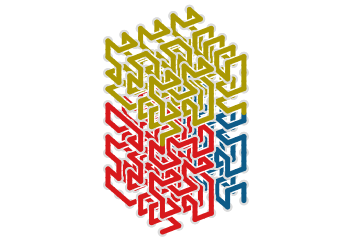
\includegraphics[width=\linewidth]{gilbert3d_eccentric_gamma_example.pdf}
		\captionof{figure}{ }
		\label{fig:gilbert3d_eccentric_gamma_example}
	\end{minipage}

  \vspace{3.0em}

	\begin{minipage}{0.49\textwidth}
		\centering
		\includegraphics[width=\linewidth]{gilbert3d_bulk_template.pdf}
		\captionof{figure}{ }
		\label{fig:gilbert3d_bulk_template}
	\end{minipage}\hfill
	\begin{minipage}{0.49\textwidth}
		\centering
		\includegraphics[width=\linewidth]{gilbert3d_bulk_example.pdf}
		\captionof{figure}{ }
		\label{fig:gilbert3d_bulk_example}
	\end{minipage}

\end{minipage}


\section*{Summary and Conclusions}
\label{sec:outlook}

The Gilbert curve provides a practical alternative to discrete Hilbert curves when the target grid has
arbitrary rectangular dimensions. This avoids padding or resampling that is otherwise required to fit
power-of-two constructions, while maintaining a recursive, locality-preserving traversal.
Such layouts are useful for cache-coherent image/volume traversal, spatial indexing, and visualization
of 1D data on 2D/3D grids \cite{anders2009, bohm2021, cortesi2011, moon2001}.

There are several natural directions for future work.
First, while our eccentric-split thresholds are simple and work well in practice, one can define more
explicit optimization criteria for when and how to switch subdivision templates.
Second, in 3D, relaxing subproblem endpoint constraints may allow constructions that further reduce
the occurrence of forced diagonal steps when one or more side lengths are odd.
Finally, more refined choices of subdivision could be explored focused on regularity metrics and/or perceptual quality.

%\section*{Conclusion}

%We presented the Gilbert curve, a simple recursive construction of Hilbert-like Hamiltonian paths on arbitrary
%2D rectangles and 3D cuboids. The construction is guided by a clean parity (color compatibility) constraint
%on corner endpoints and extends naturally from 2D to 3D.


A libre/free/open implementation for the Gilbert curve in 2D and 3D has been developed and can be downloaded from its
repository \footnote{ \label{gilbert-url} \url{https://github.com/jakubcerveny/gilbert} }.

\section*{Acknowledgments}

AI tools were used in assisting the language and readability of this paper.

{\setlength{\baselineskip}{13pt} % tighten line spacing for bibliography
\raggedright        % no right justification for References
\begin{thebibliography}{99}

  \bibitem{anders2009} S. Anders. ``Visualization of genomic data with the Hilbert curve.'' \textit{Bioinformatics}, vol.~25, no.~10, pp. ~ 1231-1235, 2009.  \url{https://doi.org/10.1093/bioinformatics/btp152}

  \bibitem{bohm2021} C. B{\"o}hm, M. Perdacher, and C. Plant ``A Novel Hilbert Curve for Cache-Locality Preserving Loops.'' \textit{IEEE Transactions on Big Data}, vol.~7, 2021, pp.~241-254

  \bibitem{cortesi2011} A. Cortesi. \textit{Visualizing binaries with space-filling curves}. 2011. \url{https://corte.si/posts/visualisation/binvis/}.

  %\bibitem{sagan1994} H. Sagan. \textit{Space-Filling Curves}, 1994 ed. Springer, 1994.

  \bibitem{hilbert1891} D. Hilbert. ``Ueber die stetige Abbildung einer Linie auf ein Fl{\"a}chenst{\"u}ck.'', \textit{Mathematische Annalen}, vol.~38, 1891, pp.~459-460

  %\bibitem{lee2025} S. Lee, K. Ma. ``HINTs: Sensemaking on large collections of documents with {\bf H}ypergraph vizualization and {\bf INT}elligent agents.'' \textit{IEEE Transactions on Visualization and Computer Graphics}, vol.~31, no.~9, 2025, pp.~5532-5546

  \bibitem{moon2001} B. Moon, H. Jagadish, C. Faloutsos, and J. Saltz. ``Analysis of the clustering properties of the Hilbert space-filling curve.'' \textit{IEEE Transactions on Knowledge and Data Engineering}, vol.~13, no.~1, 2001, pp.~124-141.

  \bibitem{munroe2006} R. Munroe. \textit{Map of the Internet}. xkcd. 2006. \url{https://xkcd.com/195/}

  %\bibitem{rong2021} Y. Rong, X. Zhang, and J. Lin. ``

  \bibitem{lutanho2003} L. Tautenhahn. \textit{Draw a space-filling curve of arbitrary size}, 2003. \url{https://lutanho.net/pic2html/draw_sfc.html}.

  \bibitem{zhang2006} J. Zhang, S. Kamata, and Y. Ueshige. ``A Pseudo-Hilbert Scan Algorithm for Arbitrarily-Sized Rectangle Region.'' \textit{Advances in Machine Vision, Image Processing, and Pattern Analysis}, Berlin, Heidelberg, 2006, pp. 290-299.
\end{thebibliography}
} % end setlength, raggedright

\begin{figure}[!htb]
  \centering
  %{\transparent{0.4}\includegraphics[width=\linewidth]{gilbert_bd50x10.pdf}}
  \includegraphics[width=0.9\linewidth]{gilbert_bd50x10.pdf}
  %\includegraphics[width=0.8\linewidth]{gilbert_fun_50x6.pdf}
  \label{fig:footerGilbert}
\end{figure}


\end{document}


